\begin{figure}[!b]
\center{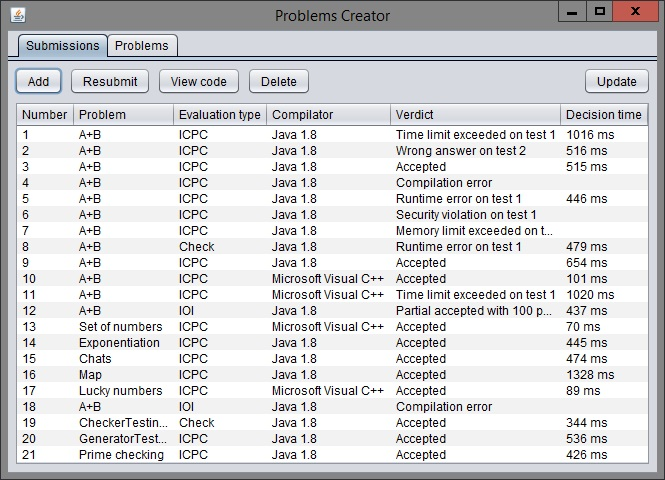
\includegraphics[scale=0.9]{screen_submissions}}
\caption{Список отправленных посылок}
\label{screen_submissions}
\end{figure}

\begin{figure}[!b]
\center{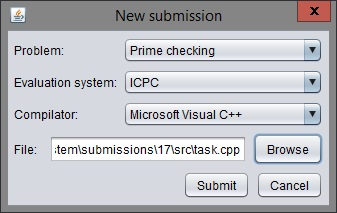
\includegraphics[scale=0.9]{screen_new_submission}}
\caption{Выбор параметров новой посылки}
\label{screen_new_submission}
\end{figure}

Рассмотрим теперь вторую вкладку главного окна приложения (рис.~\ref{screen_submissions}), на которой располагается список всех сохранённых в файловой системе посылок с вердиктами по каждой из них. Здесь можно добавить новую посылку, при этом открывается новое окно, отображённое на рис.~\ref{screen_new_submission}, в котором можно выбрать задачу, компилятор, систему оценивания и файл с исходный кодом. Также на данной вкладке можно удалить посылку, открыть её код для просмотра и перезапустить.

Мы сделаем посылку с решением, написанным на языке Java, но отличающимся от предыдущего рассмотренного решения в способе вывода множителя числа $n$. Если в прошлый раз мы выводили первое найденное число $i$, на которое $n$ делится нацело, то теперь мы будем выводить $n/i$. Ответ всё равно останется правильным, но во многих случаях окажется другим.

Запустим посылку и увидим окно, отображённое на рис.~\ref{screen_submission_results}, где видны вердикт и затраченное время по каждому тесту в задаче. Как можно видеть, такое решение также даёт вердикт <<Accepted>> на всех тестах, что говорит о корректной работе написанного нами чекера.

\begin{figure}[!h]
\center{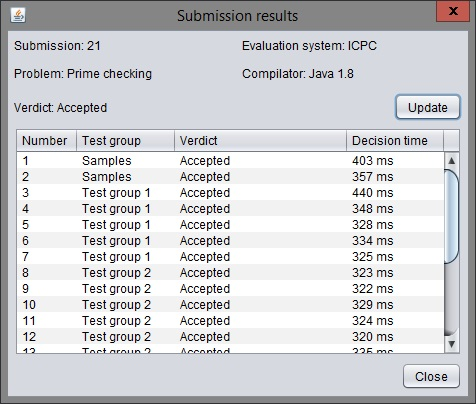
\includegraphics[scale=0.9]{screen_submission_results}}
\caption{Результаты запуска посылки на каждом тесте}
\label{screen_submission_results}
\end{figure}